% !TeX encoding = UTF-8
% 
% 作者: Yongjian.Li 澳門科技大學-畢業論文 LaTeX template-2023
% help: https://iihciyekub.github.io/must-thesis-manual
% Github: https://github.com/iihciyekub/MUST-Thesis
% Overleaf: https://www.overleaf.com/read/mjzpcxztzqzv
% Overleaf project 使用的 chrome 浏览器扩展程序 overleaf s2t/bib2bbl, 下载地址:
% https://chrome.google.com/webstore/detail/overleaf-s2tbib2bbl/icekiliecbhnockmfkehoebbkmhmapmo?hl=zh-CN
% 最後更新: 2023-04-20

\documentclass[
    writingLanguage=english, 
    % writingLanguage=chinese,
    addPageTitle=yes,
    AddDeclaration=yes,
    addMUSTlog=no,
    refUnindent=yes,
    printing=no,
]{.def/must}


% 論文基本信息,必填不能刪除
\def\shool              {Macau University of Science and Technology}
\def\cnTitle            {XXX 銀行(澳門分行)與 XXX 銀行合併之研究}
\def\cnShortTitle       {\cnTitle}% 页眉显示的中文论文短题目
\def\enTitle            {The Study on the Relationship between Social Responsibility and Organizational Trust}
\def\enShortTitle       {The Study on the Relationship between SR \& OT}% 页眉显示的英文论文短题目
\def\Name               {Name}% 名稱
\def\StudentNo          {Student No.}% 學號
\def\Faculty 	        {Faculty of Business Administration}% 所在學院
\def\Program 	        {Program}% 學位名稱
\def\Major              {Major}% 專業名稱
\def\Supervisor	        {Supervisor}% 指導老師
\def\DateofWriting		{\datea\today}% 設置論文寫作完成時間
\def\DateofDeclaration	{\dateb\today}% 設置論文原創聲明時間
\def\DateofSignature	{2023/06/30}% 設置簽署論文原創聲明的時間
\def\PublicAfterYears   {5}% 設置論文幾年後公開




 
\begin{document}


\begin{abstract@en}{keyword1,keyword1,keyword1,keyword1,}
\txtHere{1-3}
\end{abstract@en}

% 添加目錄 
\addtableofcontents


\chapter{Introduction}
\txtHere{1}
\section{Research Aim and Objectives}
\txtHere{1-2}
\subsection{Background}
\txtHere{1}\citep{abdoh2019, bordwell2013, bourdieu1990, cole1992, harvey2007, johnson2018, macdonald2020, manguel2009b, milliot9999, poff2019, villazón2011, manguel2009a}

\subsection{Current State}
\txtHere{1}

\chapter{Related Work}
\txtHere{1}
\section{Previous Studies}
\txtHere{1}
\subsection{Study 1}
\txtHere{1}
\subsection{Study 2}
\txtHere{1}
\subsection{Study 3}
\txtHere{1}
\section{Limitations of Previous Studies}
\txtHere{1}

\begin{equation}
V_0=X_0(1-T)(1-b) \sum_{t=1}^n \frac{(1+g)^t}{(1+k)^t}+\frac{X_0(1-T)(1-g)^{n+1}}{k(1+k)^n}
\end{equation}

\begin{enumerate}
\item one
\item two
\item three
\end{enumerate}
\begin{table}[htbp]
    \centering
    \caption{read csv data}
    \label{tab:mytable}
    \csvautobooktabular{data.csv} 
\end{table}


\begin{sidewaystable}[!htp]
	\caption{sidewaystable} 
	\centering
	\setlength{\tabcolsep}{10mm}
	\begin{tabular}[l]{@{}lcccccc}		
	\toprule		
	Class$^{\rm a}$ & $\gamma_1$ & $\gamma_2$$^{\rm b}$& $\langle \gamma \rangle$& $G$ & $|{ f}|$ & $\theta _{c}$ \\		
	\midrule	
        BL Lacs &5 & 36 & 7 & $-4.0$ & $1.0\times 10^{-2}$ & 10$^\circ$ \\		
        FSRQs & 5 & 40 & 11 & $-2.3$ & $0.5\times 10^{-2}$ & 14$^\circ$ \\	
        FSRQs & 5 & 40 & 11 & $-2.3$ & $0.5\times 10^{-2}$ & 14$^\circ$ \\	
        FSRQs & 5 & 40 & 11 & $-2.3$ & $0.5\times 10^{-2}$ & 14$^\circ$ \\	
        FSRQs & 5 & 40 & 11 & $-2.3$ & $0.5\times 10^{-2}$ & 14$^\circ$ \\	
        FSRQs & 5 & 40 & 11 & $-2.3$ & $0.5\times 10^{-2}$ & 14$^\circ$ \\	
        FSRQs & 5 & 40 & 11 & $-2.3$ & $0.5\times 10^{-2}$ & 14$^\circ$ \\	
        BL Lacs &5 & 36 & 7 & $-4.0$ & $1.0\times 10^{-2}$ & 10$^\circ$ \\		
        FSRQs & 5 & 40 & 11 & $-2.3$ & $0.5\times 10^{-2}$ & 14$^\circ$ \\	
        FSRQs & 5 & 40 & 11 & $-2.3$ & $0.5\times 10^{-2}$ & 14$^\circ$ \\	
        FSRQs & 5 & 40 & 11 & $-2.3$ & $0.5\times 10^{-2}$ & 14$^\circ$ \\	
        FSRQs & 5 & 40 & 11 & $-2.3$ & $0.5\times 10^{-2}$ & 14$^\circ$ \\	
        FSRQs & 5 & 40 & 11 & $-2.3$ & $0.5\times 10^{-2}$ & 14$^\circ$ \\	
        FSRQs & 5 & 40 & 11 & $-2.3$ & $0.5\times 10^{-2}$ & 14$^\circ$ \\	
	\bottomrule		
\end{tabular}
\end{sidewaystable}



\section{funation}

\begin{figure}[H]
	\centering
	\begin{tikzpicture}
	\begin{axis}
	xlabel=$x$, ylabel=$y$,
	small,
	]
	\fun[exp(-x^2-y^2)*x]
	\end{axis}
	\end{tikzpicture}
	\caption{$x\cdot \exp(-x^2-y^2)$ funation}
	\label{fig:sig}
\end{figure}
fig \ref{fig:sig} 表示$x\cdot \exp(-x^2-y^2)$ funation.






\section{mfig}
\tikzstyle{every pin}=[fill=white,draw=black,font=\small,]
\begin{figure}[H]
	\centering
	\begin{subfigure}{0.49\textwidth}
	  	\centering
		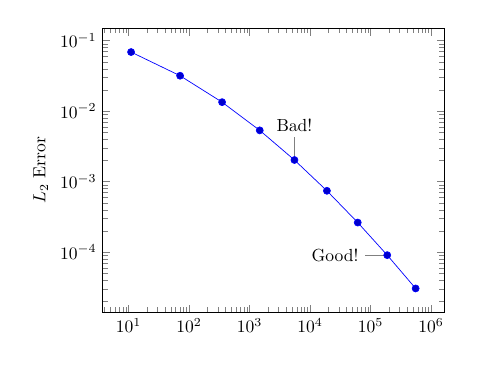
\begin{tikzpicture}[scale = 0.63276]
			\begin{loglogaxis}[
				%xlabel={\textsc{Dof}},
				ylabel={$L_2$ Error},
				]
				\addplot coordinates {
					(11, 6.887e-02)
					(71, 3.177e-02)
					(351, 1.341e-02)
					(1471, 5.334e-03)
					(5503, 2.027e-03)
					(18943, 7.415e-04)
					(61183, 2.628e-04)
					(187903, 9.063e-05)
					(553983, 3.053e-05)
				};
				\node [coordinate,pin=above:{Bad!}]
				at (axis cs:5503,2.027e-03) {};
				\node [coordinate,pin=left:{Good!}]
				at (axis cs:187903,9.063e-05) {};
			\end{loglogaxis}
		\end{tikzpicture}
		\caption{A subfigure}
		\label{fig:sub1}
	\end{subfigure}
	\hfill
	\begin{subfigure}{.49\textwidth}
		\centering
		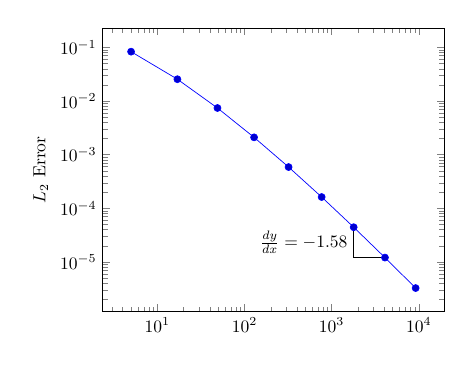
\begin{tikzpicture}[scale = 0.63276]
			\begin{loglogaxis}[
				ylabel=$L_2$ Error,
				]
				\draw
				(1793,4.442e-05)
				|- (4097,1.207e-05)
				node [near start,left]
				{$\frac{dy}{dx} = -1.58$};
				\addplot coordinates {
					(5, 8.312e-02)
					(17, 2.547e-02)
					(49, 7.407e-03)
					(129, 2.102e-03)
					(321, 5.874e-04)
					(769, 1.623e-04)
					(1793, 4.442e-05)
					(4097, 1.207e-05)
					(9217, 3.261e-06)
				};
			\end{loglogaxis}
		\end{tikzpicture}
		\caption{A subfigure}
	  	\label{fig:sub2}
	\end{subfigure}\\

	\begin{subfigure}{.49\textwidth}
		\centering
		\includegraphics[width=.5\linewidth]{\resourcePath eg05}
		\caption{A subfigure}
		\label{fig:sub3}
	\end{subfigure}
	\begin{subfigure}{.49\textwidth}
		\centering
		\includegraphics[width=.5\linewidth]{\resourcePath eg06}
		\caption{A subfigure}
		\label{fig:sub4}
	\end{subfigure}
	\caption{A figure with two subfigures}
	\label{fig:sub}
\end{figure}
 
In the example above, the subfigures \ref{fig:sub1}, \ref{fig:sub2}, \ref{fig:sub3}, and \ref{fig:sub4} represent subfigures 1, 2, 3, and 4, respectively.


\chapter{數學公式}
\begin{equation}
\label{eq1}
e^{\pi i}+1=0
\end{equation}
\begin{align}
2 y & =d\label{eq:IntoSection}\\
3 y & =cx+d\\
4 y_{12} & =bx^{2}+cx+d\\
5 y(x) & =ax^{3}+bx^{2}+cx+d
6 
\end{align}
\begin{equation}
2 x=\left\{ \begin{array}{cl}
3 0 & \textrm{if }A=\ldots\\
4 1 & \textrm{if }B=\ldots\\
5 x & \textrm{this run  text.}\end
{array}\right.
\end{equation}       


\subsection{算法表}
\begin{algorithm}[H]
    \fz[10][0.25]
	\SetAlgoVlined %設置帶水平線的連線
	\PrintSemicolon
	\KwData{document set $D :=\{d_1,d_2,\cdots,d_i\}$, term vector $d_1 =\{t_1,t_2,\cdots,t_j\}$
	}
	\KwResult{top6000,High TF-IDF Frequency Keywords}
	\Begin{
	term matrix:$\ \mathcal{L};  \hfill /* \textit{Initial value is empty ($j \times i$)} */$\\
	counter:$\ i =0, j=0;$\\
	    \For{$d  \in D$}{
	        $ i\ $++;\\ 
	        \For {$t \in d$} {
	                $ j\ $ ++;\\[-2mm]
	                $ w_{i,j} = \text{tf}(t,d)\cdot \text{idf}(t,D) = \dfrac{f_{t,d}}{n_d} \cdot \log \dfrac{N}{|\{d \in D: t \in d\}|};$\\
	                $ \mathcal{L}_{i,j}$.Append($t,w_{i,j}$);\\
	            }
            $\mathcal{L}_{i,j}$.Sort(by:$w_{i,j}$)[:10];   \hfill /* \textit{descending rank and retain the top 10.}*/\\
            $\mathcal{L}_{i,j}$.Reindex(); \hfill /* \textit{reset the index.}*/
	        }
   \vspace{-1.5mm} term matrix: $\mathcal{L}= 
    \left[\begin{array}{llll}
    t'_{1,1} & t'_{1,2} & \cdots & t'_{1,10}  \\[-2mm]
    \vdots &\vdots &\vdots & \vdots\\[-1mm]
    t'_{j,1} & t'_{j,2} & \cdots & t'_{j,10}  \\[-1mm]
    \end{array}\right]
    $    \hfill /* \textit{print $\mathcal{L} \ (10\times j)$  result} */\\[0.5em]
    \nlset{Note$^\star$ \ \ \ \ \  }   \textbf{OutputFile: \textbf{File}$^{(1,\divideontimes)}$ } \\[0.5em] 
    \For {$ t' \in \mathcal{L}  $}{
    $i,j \leftarrow t'$ .index()\\[-1mm]
        $w_{i,j} = \text{tf}(t', \mathcal{L}  ) =  \dfrac{f_{t'} }{10 \cdot j} ;$           \hfill /* \textit{where $f_{t'}$ is the raw count of a term $t'$ in $\mathcal{L} $ }*/ \\
    }
     \nlset{Remark$^\star$ \ \ \ \ \  }  $\mathcal{L} $.Sort(by:$w_{i,j}$)[:6000];   \hfill /* \textit{descending rank and retain the top 6000.}*/\\[0.5em]
         \nlset{Note$^\star$ \ \ \ \ \  }   \textbf{OutputFile: \textbf{File}$^{(2,\divideontimes)}$ }  \\[0.5em]
    \textbf{End}
    }	
	\caption{Text Mining: Keyword Extraction Algorithm}
\end{algorithm}

 





\chapter{Methodology}
\txtHere{1}
\section{Research Design}
\txtHere{1}
\subsection{Experimental Design}
\txtHere{1}
\subsection{Sampling Method}
\txtHere{1}
\section{Data Collection}
\txtHere{1}
\subsection{Data Sources}
\txtHere{1}
\subsection{Data Collection Procedures}
\txtHere{1}
\section{Data Analysis}
\txtHere{1}
\subsection{Statistical Analysis}
\txtHere{1}
\subsection{Qualitative Analysis}

\chapter{Results}
\txtHere{1}
\section{Descriptive Statistics}
\txtHere{1}
\subsection{Frequencies}
\txtHere{1}
\subsection{Measures of Central Tendency}
\txtHere{1}
\subsection{Measures of Dispersion}
\txtHere{1}
\section{Inferential Statistics}
\txtHere{1}
\subsection{Hypothesis Testing}
\txtHere{1}
\subsection{Regression Analysis}
\txtHere{1}
\subsection{Factor Analysis}
\txtHere{1}

\chapter{Discussion}
\txtHere{1}
\section{Interpretation of Results}
\txtHere{1}
\subsection{Implications of Results}
\txtHere{1}
\subsection{Limitations of Study}
\txtHere{1}
\section{Contributions to the Field}
\txtHere{1}
\subsection{Recommendations for Future Research}
\txtHere{1}

\chapter{Conclusion}
\txtHere{1}
\section{Summary of Findings}
\txtHere{1}
\section{Conclusions}
\txtHere{1}
\section{Limitations of Study}
 \txtHere{1}
\txtHere{1}
\section{Implications for Practice}
\txtHere{1}




% 請確保bib 文件名稱為 ref.bib, 利用js文件處理後的bbl文件名稱為 ref.bbl
\addreference


\begin{appendix}

\end{appendix}


\begin{acknowpage}

\end{acknowpage}




% 填寫個人簡歷
\begin{addcvpage}
% 設置入學時間
\addedudate{Sept, 2019}

% 填寫教育經歷,注意內容以逗號作分隔,
\addeduItem{2009.16-2012.13,Macau University of Science and Technology, Faculty of Business, Taipa Island, Macau, China.}
\addeduItem{2009.16-2012.13,Macau University of Science and Technology, Faculty of Business, Taipa Island, Macau, China.}
\addeduItem{2009.16-2012.13,Macau University of Science and Technology, Faculty of Business, Taipa Island, Macau, China.}


%增加學術文章
\addpaperItem{ 
    \item  Macau University of Science and Technology, Taipa Island, Macau, China.,
    \item Macau University of Science and Technology, Taipa Island, Macau, China.,
}


% 增加項目
\addprojectItem{
    \item 中國澳門氹仔島澳門科技大學,商學院商學院
    \item  商學院商學院商學院中國澳門氹仔島澳門科技大學,商學院商學院商學院商學院商學院中國澳門氹仔島澳門科技大學,商學院商學院商學院商學院商學院
}
\end{addcvpage}








\end{document}